
\renewcommand{\arraystretch}{1.5} % Default value: 1

%%% Write here
%%%%%%%%%%%%%%%%%%%%%%%%%%%%%%%%%%%%%
\section{Introduction}
Optical polarimetry, ever since its discovery, has played important roles in gaining fundamental understanding of the nature of electromagnetic waves and answering some of the key questions related to the physics of light. Traditional polarimetry has also long being pursued for numerous practical applications in various branches of science and technology. Quantification of protein properties in solutions, testing of chiral (asymmetric) purity of pharmaceutical drugs, remote sensing in meteorology and astronomy, optical stress analysis of structures, and crystallography of biochemical complexes are just a smattering of its diversified uses. This particular polarimetry experiment involves determination of two important polarization characteristics of medium, namely, the linear retardance and optical rotation (defined subsequently), which has many practical applications.
%%%%%%%%%%%%%%%%%%%%%%%%%%%%%%%%%%%%%
\section{Objective}
The main opjective of this experiment is to determine of linear retardance and Optical rotation of a Spatial Light Modulator (SLM) measuring various Stokes vector elements
%%%%%%%%%%%%%%%%%%%%%%%%%%%%%%%%%%%%%
\section{Equipment Required}
The following equipments are required for this experiment
\begin{itemize}
    \item Diode laser (650 nm)
    \item Spatial Light Modulator (SLM)
    \item Two Polarizer with mounts
    \item Photo-detector
    \item Optical table and mounts
    \item Computer with software for data acquisition and analysis
    \item Power supply for the SLM
    \item Glass plate with stage having rotational circular scale(in degree)
\end{itemize}
%%%%%%%%%%%%%%%%%%%%%%%%%%%%%%%%%%%%%
\section{Theory}


\subsection{Basics of Polarization}
Christian Huygens was the first to suggest that light was not a scalar quantity based on his work on the propagation of light through crystals; it appeared that light had `sides' in the words of Newton. This vectorial nature of light is called polarization \cite{Goldstein2003PolarizedLight}.

In a Cartesian system the components $u_x(\mathbf{r},t)$ and $u_y(\mathbf{r},t)$ are said to be the transverse components, and the component $u_z(\mathbf{r},t)$  is said to be the longitudinal component when the propagation is in the z direction. Thus we can write

\begin{subequations}
\begin{align}
u_x(\mathbf{r},t) &= u_{0x}\cos(\omega t - \mathbf{k}\cdot\mathbf{r} + \delta_x), \label{eq:u_x}\\
u_y(\mathbf{r},t) &= u_{0y}\cos(\omega t - \mathbf{k}\cdot\mathbf{r} + \delta_y), \label{eq:u_y}\\
u_z(\mathbf{r},t) &= u_{0z}\cos(\omega t - \mathbf{k}\cdot\mathbf{r} + \delta_z). \label{eq:u_z}
\end{align}
\end{subequations}

Experimentally found that light consisted only of the transverse components \cref{eq:u_x} and \cref{eq:u_y}. If we take the direction of propagation to be in the z direction, then the optical field in free space must be described only by \cref{eq:u_x} and \cref{eq:u_y}. where $u_{0x}$ and $u_{0y}$ are the maximum amplitudes and $\delta_x$ and $\delta_y$ are arbitrary phases. These two \cref{eq:u_x} and \cref{eq:u_y} are are spoken of as the polarized or polarization components of the optical field. Now, the transverse components are represented by

\begin{subequations}\label{eq:E_trans}
\begin{align}
E_x(z,t) &= E_{0x}\cos(\tau+\delta_x), \label{eq:E_x}\\
E_y(z,t) &= E_{0y}\cos(\tau+\delta_y), \label{eq:E_y}
\end{align}
\end{subequations}

where $\tau=\omega t-kz$ is the propagator. The subscripts $x$ and $y$ refer to the components in the $x$ and $y$ directions. $E_{0x}$ and $E_{0y}$ are the maximum amplitudes, and $\delta_x$ and $\delta_y$ are the phases, respectively. As the field propagates, $E_x(z,t)$ and $E_y(z,t)$ give rise
to a resultant vector. This vector describes a locus of points in space, and the curve generated by those points will now be derived. In order to do this \cref{eq:E_x} and \cref{eq:E_y} are written as

\begin{subequations}
\begin{align}
\frac{E_x}{E_{0x}} &= \cos\tau\cos\delta_x- \sin\tau\sin\delta_x, \\
\frac{E_y}{E_{0y}} &= \cos\tau\cos\delta_y - \sin\tau\sin\delta_y. 
\end{align}
\end{subequations}


\begin{figure}[H]
    \centering
    \begin{subfigure}[t]{0.45\textwidth}
        \centering
        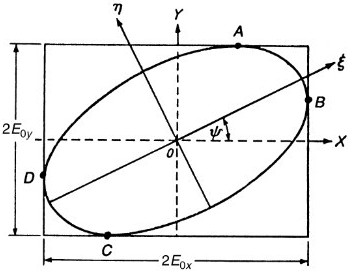
\includegraphics[width = \textwidth]{Image/polarization2.jpg}
        \caption{An elliptically polarized wave and the polarization ellipse}
        \label{fig:polarization_ellipse}
    \end{subfigure}
    \hfill
    \begin{subfigure}[t]{0.45\textwidth}
        \centering
        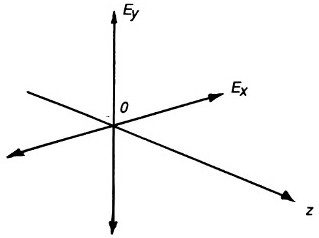
\includegraphics[width = \textwidth]{Image/polarization1.jpg}
        \caption{Propagation of the transverse optical field}
        \label{fig:propagation_wave}
    \end{subfigure}
    \caption{Polarization of light}  
    % \label{fig:enter-label}
\end{figure}



Hence,

\begin{subequations}\label{eq:polarization-relations}
\begin{align}
\frac{E_x}{E_{0x}}\sin\delta_y
-\frac{E_y}{E_{0y}}\sin\delta_x
&= \cos\tau\,\sin(\delta_y-\delta_x),
\label{eq:cos-relation}\\
\frac{E_x}{E_{0x}}\cos\delta_y
-\frac{E_y}{E_{0y}}\cos\delta_x
&= \sin\tau\,\sin(\delta_y-\delta_x).
\label{eq:sin-relation}
\end{align}
\end{subequations}

Squaring \eqref{eq:cos-relation} and \eqref{eq:sin-relation} and adding gives

\begin{subequations}\label{eq:polarization-ellipse}
\begin{align}
\frac{E_x^2}{E_{0x}^2}
+\frac{E_y^2}{E_{0y}^2}
-2\frac{E_x}{E_{0x}}\frac{E_y}{E_{0y}}\cos\delta
&=\sin^2\delta,
\label{eq:ellipse-equation}\\
\delta &= \delta_y-\delta_x.
\label{eq:phase-difference}
\end{align}
\end{subequations}

\cref{eq:ellipse-equation} is recognized as the equation of an ellipse and shows that at any instant of time the locus of points described by the optical field as it propagates is an ellipse (see \cref{fig:polarization_ellipse}). This behavior is spoken of as optical polarization, and \cref{eq:ellipse-equation} is called the \emph{polarization ellipse} \cite{Goldstein2003PolarizedLight}.

Also, we can write some more parameters of ellipse in terms of $\delta$ and $\alpha$ where $\tan{\alpha} = E_{0y}/E_{0x}$

\begin{subequations}
    \begin{align}
    \tan 2\psi &= (\tan 2\alpha)\cos\delta, 
    \qquad 0 \le \psi \le \pi, \\
    \sin 2\chi &= (\sin 2\alpha)\sin\delta,
    \qquad -\frac{\pi}{4} \le \chi \le \frac{\pi}{4}.
    \end{align}
\end{subequations}

\subsection{Stokes Vector and Muller Matrix}

%%%%%%%%%%%%%%%%%%%%%%%%%%%%%%%%%%%%%
\section{Set up and Procedure}
This experiment has two parts. In the first part, we did measure the angles of polarizers (P1 and P2) for Horizontal polarization. And in the later part we did Stokes polarimetry for SLM. 
\subsection*{Part 1}


\begin{figure}[H]
    \centering
    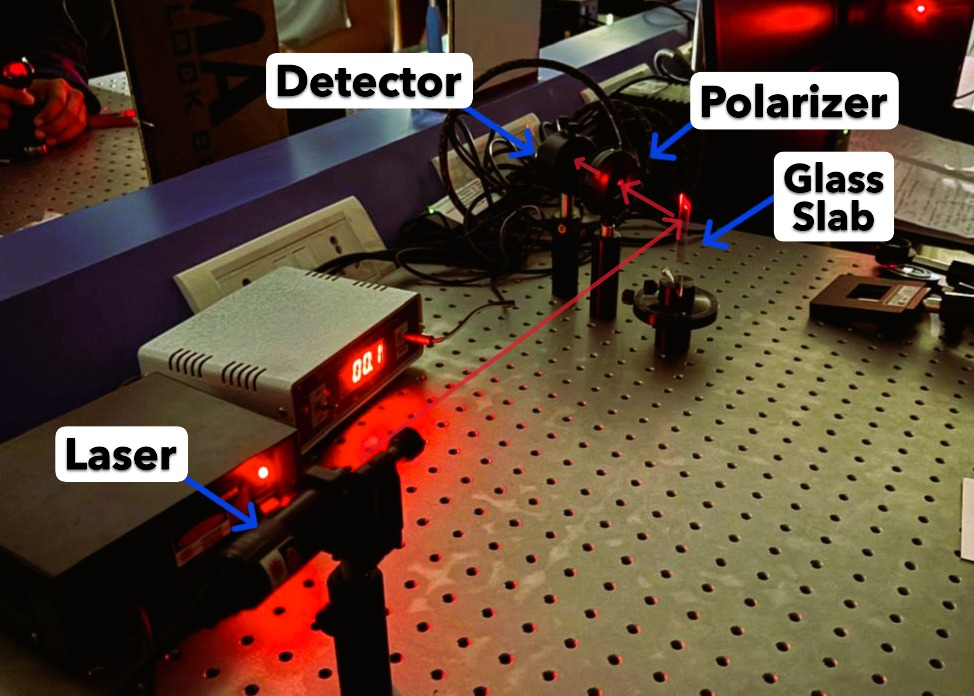
\includegraphics[width = 0.6\textwidth]{Image/part1.JPG}
    \caption{Setup to find the axis of the first polarizer (P1) using Brewster's angle approch}
\end{figure}

\begin{figure}[H]
    \centering
    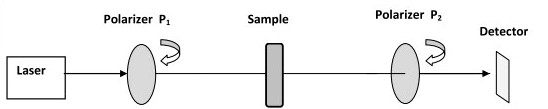
\includegraphics[width = \textwidth]{Image/schematic.jpg}
    \caption{Schematic of the final setup}
\end{figure}

\begin{figure}[H]
    \centering
    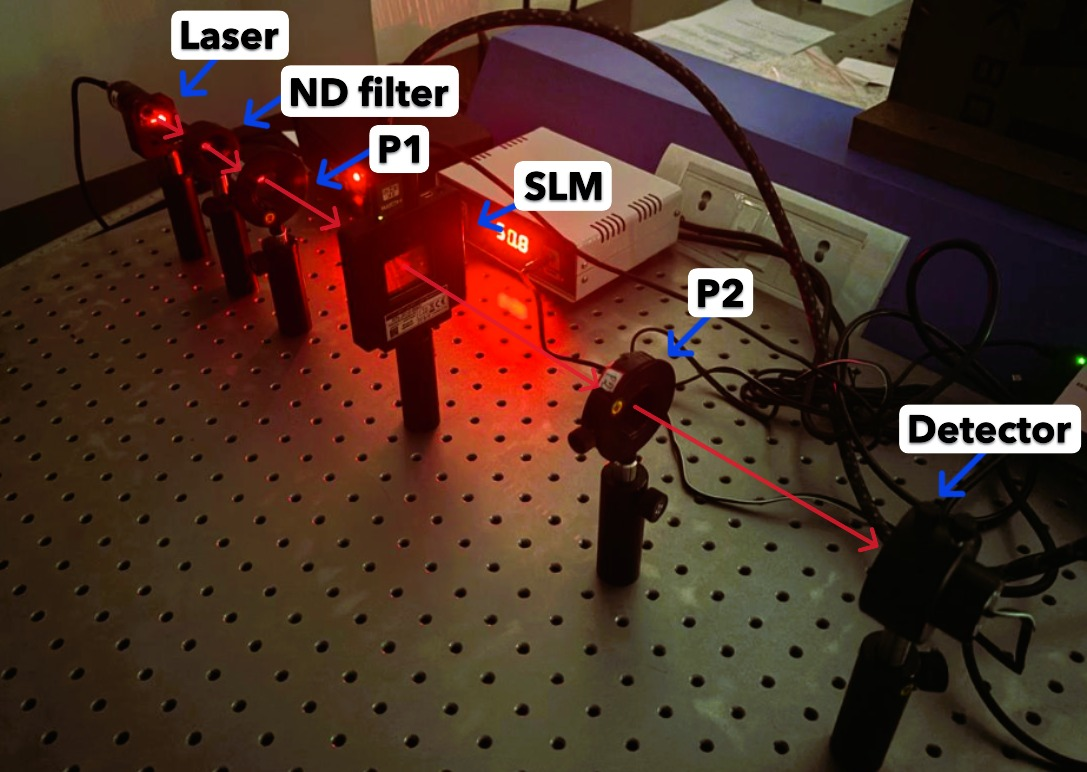
\includegraphics[width = 0.8\textwidth]{Image/part2.JPG}
    \caption{Final setup to find the Stokes measurement}
\end{figure}

%%%%%%%%%%%%%%%%%%%%%%%%%%%%%%%%%%%%%
\section{Data analysis and calculation} 
%%%%%%%%%%%%%%%%%%%%%%%%%%%%%%%%%%%%%
\section{Conclusion}
%%%%%%%%%%%%%%%%%%%%%%%%%%%%%%%%%%%%%